\chapter{Grammar and Induction}

\begin{quote}
``... small number
of symbols and their grammar are enough to capture the huge
variety of equations...''
\end{quote}

Ask yourself how you know what to do when  
substituting for $x\defeq 7$ in $x(x+3)^{2}$.
(Using $\defeq$ indicates an assignment, not an equality variable.)
Whether obvious or not, we start by parsing the grammar.  We can make this 
visual with a \emph{parse tree}.
\begin{center}
    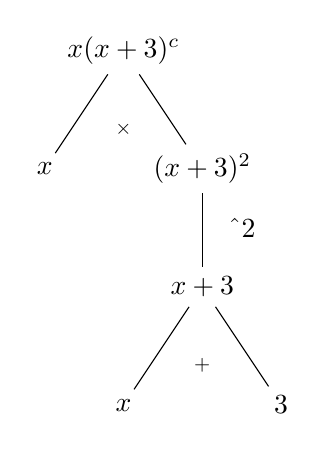
\begin{tikzpicture}[yscale=0.75]
        \node (f) at (0,0) {$x(x+3)^c$};
        \node[below of=f,scale=0.75] {$\times$};
        \node (x1) at (-1,-2) {$x$};
        \node (sqrt1) at (1,-2) {$(x+3)^{2}$}; 
        % \node[below of=sqrt1,scale=0.75] {$\circ$};
        \node (su) at (1.5,-3) {\textasciicircum 2};
        \node (u) at (1,-4) {$x+3$};
        \node (x2) at (0,-6) {$x$};
        \node[below of=u,scale=0.75] {$+$};
        \node (three) at (2,-6) {$3$};
        % \node (x3) at (0,-8) {$x$};
        % \node (x4) at (2,-8) {$x$};
        % \node[below of=x2,scale=0.75] {$\times$};

        \draw[-] (f) -- (x1);
        \draw[-] (f) -- (sqrt1);
        % \draw[-] (sqrt1) -- (su);
        \draw[-] (sqrt1) -- (u);
        \draw[-] (u) -- (x2);
        \draw[-] (u) -- (three);
        % \draw[-] (x2) -- (x3);
        % \draw[-] (x2) -- (x4);

    \end{tikzpicture}
\end{center}
Starting at the top, apply individualized 
rules for each step.  Substitute in a product $MN[x\defeq 7]$ you compute 
$M[x\defeq 7]N[x\defeq 7]$,
sometimes denoted by a ``leads to'' relation $\leadsto$. So,
with $M+N$ we can write,
\[
    (M+N)[x\defeq 7]\leadsto M[x\defeq 7]+N[x\defeq 7]
\]
At the end we finish off with rules like $3[x\defeq 7]\leadsto 3$ and $x[x\defeq 7]\leadsto 7$.
If we use $x\defeq 3$ or $x\defeq t$ we use the same procedure.

You may have been taught induction through stories of falling 
dominos.  Good.  But what if induction was more like climbing, 
and the domino illustration was bottling up the experience
of climbing stairs?  Surely its more fun to climb trees and mountains.
Climbing can go up (induct) or down (recurse) by some perspective of up/down.
So substitution was recursing, climbing down our tree to its tips.  The constants 
and single variables were bases cases.  The branches were explored independently.

\section{Grammar}
Climbing could find many routes, even go in cycles, but 
substitution happened upon a tree, why?  Well the parsing 
formulas is the same thing you do when you diagram a sentence in grammar school, only with
English you can sometimes get cycles.  
\begin{center}
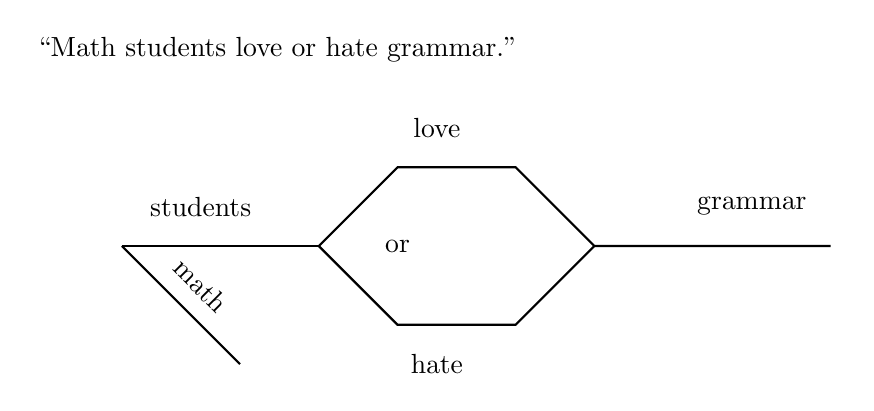
\begin{tikzpicture}
    \node[text width=4in] at (0,2) {``Math students love or hate grammar.''};
    \node at (-3,0) {students};
    \node[rotate=-45] at (-3,-1) {math};
    \node at (-0.5,-0.5) {or};
    \node at (0,1) {love};
    \node at (0,-2) {hate};
    \node at (4,0) {grammar};

    \draw[thick] (-4,-0.5) -- ++(2.5,0);
    \draw[thick] (-4,-0.5) -- ++(1.5,-1.5);
    \draw[thick] (-1.5,-0.5) -- ++(1,1) -- ++(1.5,0) -- ++(1,-1) -- ++(3,0);
    \draw[thick] (-1.5,-0.5) -- ++(1,-1) -- ++(1.5,0) -- ++(1,1);

\end{tikzpicture}
\end{center}
That we got a tree in math formulas is owed to the fact
that the grammars for mathematics are free of relations, what Chompsky's 
\emph{Syntactic Structure} calls
\emph{context-free} grammars.\footnote{
    If an algebraist starts a talk with story that ``...It was thought  all natural 
    languages were context-free until some obscure dialect in the alps or Africa was found...'', 
    then tune out until they return to equations.  
    Linguist never had such illusions. Even English is not context-free, read  James Higginbotham.}  

Induction in context-free grammars is to build up (you may need to rotate your drawing to think of it as ``up'')
taking fixed types of leaves and combining them with branches till we reach the root.
So to specify a context-free grammar we specify the atoms of our language.
For natural numbers we can used digits $0,1,\ldots, 9$.  Then we write down patterns of how to 
combine digits.  The separate cases are designated by the auxiliary symbol `$|$' (which reads as ``or'').  Each rule 
is given an name called a \emph{token} (or \emph{tag}) and denoted \lstinline{<Name>}.
Since the Walrus $\defeq$ is our assignment of variables, we use the ``astonished Walrus'' $::=$ as assignment of token rules.
Listing~\ref{lst:nat-grammar} shows the grammar for natural numbers as digits.
\begin{lstfloat}
\begin{lstlisting}[mathescape]
     <PosDig> ::= 1 | 2 | 3 | 4 | 5 | 6 | 7 | 8 | 9 
      <Digit> ::= 0 | <PosDig>
       <Nat>  ::= <Digit> | <PosDig><Nat>
\end{lstlisting}
\caption{The grammar for natural numbers.}
\label{lst:nat-grammar}
\end{lstfloat}

The natural number grammar is said to \emph{accept} $0$ as a digit, written ``0:Digit'' and also as 
a Nat, ``0:Nat''.  It also accepts 541:Nat and 10:Nat but it rejects ``01:Nat''
as that case does not exist as a rule for any token in this grammar.  Deciding to accept or 
reject is recursion, work down until you can decide.  Induction can only ever deliver a sentence 
accepted by the grammar.  The strings accepted by our grammar are known as the  \emph{language}
for that grammar.  They are teh source of one of the most important algebras out there, the free algebras.

\begin{center}
\begin{tikzpicture}
    \node at (-3.5,0) {\begin{tikzpicture}
        \node (10) at (0,0) {10:Nat};
        \node (1) at (-2,-2) {1:PosDig};
        \node (0n) at ( 2,-2) {0:Nat};
        \node (0d) at ( 2,-4) {0:Digit};
        \draw[thick] (0d) -- (0n) -- (10) -- (1);
        \node[below of=10,scale=0.75,text width=0.6in] {Nat case 2};
        \node[scale=0.75,text width=0.6in] at ( 1.5,-3) {Nat case 1};
    \end{tikzpicture}};
    \node at (3.5,0) {\begin{tikzpicture}
        \node (01) at (0,0) {01:Nat};
        \node (1) at ( 2,-2) {1:PosDig};
        \node (0n) at (-2,-2) {0:Nat};
        \node (0d) at (-2,-4) {0:Digit};
        \draw[thick,dashed] (0n) -- (10) -- (1);
        \draw[thick] (0d) -- (0n);
        \node[below of=01,scale=0.75,text width=0.6in] {no case!};
        \node[scale=0.75,text width=0.6in] at (-1.3,-3) {Nat case 1};
    \end{tikzpicture}};
\end{tikzpicture}
\end{center}

Having a tree makes moving about the nodes a unique process, because trees 
have a unique path between any to vertices.  So if we root the tree at the start 
we have a unique path to get to the leaves, where we place the base cases.  
Recursion on trees is so special it has its own name: \emph{traversing}.
Of course, if we are doing one step at a time we still have choices: first go left, then go right, and 
etc.  That is our next concern.



\begin{remark}
The symbols \lstinline{::=}, \lstinline{<Token>} and \lstinline{|} are 
Backus-Naur Form (BNF) notation, which is popular 
in computer science.  It is actually subject to its own gammar, admittedly 
basic and fixed in length.  But you can be forgiven for wondering if this is 
all circular reasoning.  When this occurs, mathematicians like to attach 
the word \emph{meta}, which means literally ``self-referential''.
So BNF would be called a \emph{meta-language}. Like axioms and postulates 
these are choices and beliefs, they do not survey all possibilities.

These ideas under different notation were written 
down in 600 BC by Panini's rules of Sanskrit grammar.  
Good ideas get rediscovered;
great ideas get stolen.
\end{remark}
